\documentclass[a4paper,12pt]{article}
\usepackage{array}
\usepackage{listings}
\usepackage{graphicx}
\graphicspath{ {./images/} }

\setlength{\tabcolsep}{18pt}
\renewcommand{\arraystretch}{1.2}


\begin{document}
\title{Zusammenfassung Datennetze 1}
\author{Mathis Hermann}
\date{\today}
\maketitle
Diese Zusammenfassung ist anhand der Lernziele aufgebaut. Dementsprechend sind nicht ganz alle Themen der Vorlesung enthalten.

\section{Übersicht über Datennetze}



\paragraph{Client-Server Paradigma} -- Meiste Kommunikation; Daten auf ServerM User können Daten auf Server bearbeiten

\paragraph{Peer-to-Peer Paradigma} -- Rechner kann Server und Client sein; Einfach aufzusetzen, weniger Komplexität, weniger Kosten; Keine zentralisierte Administration, nicht so sicher, nicht skalierbar

\paragraph{LAN und WAN} -- Es gibt verschiedene Typen von Netzen:\\
Kriterien:
\begin{itemize}
\item Kanalzugang
\begin{itemize}
\item Multiaccess Netze
\item Punkt-zu-Punkt Netze
\end{itemize}
\item Ausdehnung
\begin{itemize}
\item LAN (sind immer Multiaccess Netze)
\item WAN (traditionell: Punkt-zu-Punkt Netze; neu auch Multiaccess Netze)
\end{itemize}
\end{itemize}

\paragraph{Begriffe}
\begin{center}
\begin{tabular}{ | m{2.5cm} | m{9cm} | } 
Begriff & Erklärung\\ 
\hline
Client & Wird ein- und ausgeschaltet; wechselt IP; stellt Anfrage an Server\\
Server & Ein Programm, das immer läuft; fixe IP; meistens DNS- Eintrag; läuft ununterbrochen und wartet auf Anfragen\\
LAN & Local-Area Network; Enthält  Endgeräte; Medium-Access Control; \emph{multi-access} Netz \\
WAN &Wide-Area Network; Keine Endgeräte; \emph{point-to-point} Leitungen\\
Physikalische Darstellung & Definiert die physikalischen Verbindungen und Konfigurationen; Zeigt welches Gerät sich wo befindet und mit welchem verbunden ist\\
Logische Darstellung & Darstellung Ebene 3; Netze werden gezeichnet\\
Switch & Layer 2 Kommunikation; leitet Rahmen innerhalb eines Netzwerkes weiter\\
Router & Layer 3; Verbindet IP-Netze; leitet Pakete von einem Netz in ein anderes\\
Konvergierte Netze & Ein Netz für alle Dienste; single point of failure im Netz durch Komplexität; billiger im Unterhalt\\
Downstream & (Stärke der) Leitung von ISP zu Konsument\\
Upstream & (Stärke der) Leitung von Konsument zu ISP\\
QoS & Dienstgüte\\
Leitungs-vermittlung & Endgerät baut Leitung zu Ziel auf; feste Bandbreite wird reserviert in festem zeitlichen Rahmen; starke QoS; geringer Durchsatz (stark begrenzt in Bandbreite); sicher\\
Paket-vermittlung & Nachricht wird segmentiert; Pakete werden anhand der Informationen (Absender, Empfänger) verteilt; gute Ausnützung der Bandbreite; nicht so sicher; viel Overhead bei Paketen - nicht so effizient\\
\end{tabular}
\end{center}

\paragraph{Netzwerkelemente und deren Funktion} -- Netzwerkelemente sind \emph{Endgeräte} (Computer, Laptop, Drucker, Tablet); \emph{Zwischengeschaltete Geräte} (Router, Switch) ; \emph{Anschlussleitung} (Wireless Media, LAN Media, WAN Media)

\paragraph{Dedizierte und Konvergierte Netze} -- verschiedene Dienste über das Internet\\
\emph{Dedizierte Netze} -- Spezifische Netze für entsprechende Anwendungen; \emph{Konvergente Nezte} -- Ein Netz für alle Dienste;

\paragraph{Logische und Physikalische Darstellung von Netzwerken} -- \emph{Logische Sicht} Beschreibt welche IP-Netze (Benutzergruppen) es gibt; \emph{Physikalische Sicht} Beschreibt wo welches Netzelement befindet

\paragraph{Grundanforderungen des Internets}
Kriterien für zuverlässige Netze:

\begin{itemize}
\item Fehlertoleranz (z.B. bei Leitungunterbruch)
\item Skalierbarkeit
\item Dienstgüte
\item Sicherheit (e.g. Abhören oder Manipulation der Daten)
\end{itemize}

\paragraph{Anforderung verschiedener Anwendungen an die verschiedenen Parameter der Dienstgüte}

\begin{center}
\begin{tabular}{ | m{1.2cm} |m{1.2cm}|m{2cm}|m{1cm}|m{2cm}| } 
An-wendung & Durch-satz & Ver-zögerung & Jitter & Paket-vermittlung\\ 
\hline
Web & Hoch & Gering & Gering & Hoch\\
E-Mail & Gering & Gering & Gering & Gering\\
Sprache & Gering & Hoch & Hoch & Gering (VoIP)\\
Video & Mittel & Hoch & Hoch & Gering\\
\end{tabular}
\end{center}

\newpage
\paragraph{Unterschied: Leitungsvermittlung und Paketvermittlung} \emph{Leitungsvermittlung} -- Viele mögliche Pfade; ein Pfad wird gewählt pro Call; Wenn ein Call etabliert ist, geht alle Kommunikation über diesen Pfad; Eine Leitung ist bestimmt für die gesamte Dauer des Calls\\
\emph{Paketvermittlung} -- Viele verschiedene Pfade können verwendet werden, um individuelle Pakete zum Ziel zu routen; kein fixer Pfad; Pakete werden entsprechend des besten Pfades zur Zeit geroutet \\

\newpage
\section{Konfiguration von Netzen}
\paragraph{Zugänge zum Betriebssystem IOS von Cisco} -- Hauptsächlich über drei HW-Schnittstellen kann ein Router konfiguriert werden: \emph{1)} Console Port, blau: Management Port für lokale Konfiguration (Lokale Konsole, Serial), \emph{2)} Auxiliary Port, schwarz: Management Port für entfernte Konfiguration ("Remote out-of-band", wird kaum mehr genutzt), \emph{3)} LAN Anschlüsse, gelb: Remote Management ("inband management") mit SSH, Telnet.



\paragraph{Kommandos IOS} -- Drei verschiedene Arten von Kommandos in IOS: \emph{1)} Betriebskommandos ("ping"; Speichern von Konfiguration etc), \emph{2)} Konfigurationskommandos (zur Konfiguration eines Interfaces, Passwort etc.), \emph{3)} Statusabfragen.

\paragraph{Kommandostruktur von IOS} -- Es gibt vier verschiedene Modi im IOS: \emph{1)} User Mode, \emph{2)} Privileged Mode, \emph{3)}Global Config Mode, \emph{4)} Config Mode (und Sub-Menus).


\paragraph{Wie wird ein Router oder Switch out-of-the-box konfiguriert?}
\begin{lstlisting}
Router>enable	// exec zu privileged mode
Router#configure terminal // in Konfigurationsmodus
Router(config)#interface FastEthernet 0/0
// IF-Konfigurationsmodus - Interfaces konfigurieren

Router(config-if)# // Ebene zurueck
Router(config)#	// Ebene zurueck
Router#disable	// zurueck in den user mode
Router>

// Hilfe im IOS

Router# cl? //liste von commands, die mit "cl" starten
clear clock

Router#clock set ? // next possible arguments
  hh:mm:ss	Current Time
  
Router#clock set 19:50:00 ? // mehrere Argumente
  <1-31>	Day of the month
  MONTH		Month of the year

Router#clock set 19:50:00 25 June 2022

// Konfiguration auslesen
Router#show running-config
	// laufende Konfiguration aus RAM

Router#show startup-config
	// Abgespeicherte Konfiguration aus NVRAM
	
Router#show flash // Inhalt von Flashspeicher
Router#show version // Informationen zum aktuellen IOS
Router#show ip interface brief // Zustand aller IFs
\end{lstlisting}

\paragraph{Grundkonfiguration für Router und Switch} Eine Grundkonfiguration beinhaltet:
\begin{itemize}
\item Hostname
\item Einschränkung des Zugangs zu Netzelementen mit Passwörtern
	\begin{itemize}
	\item Lokales Einloggen (Console)
	\item Entferntes Einloggen (Telnet, SSH)
	\item Übergang user mode zu privileged mode
	\end{itemize}
\item Rechtlicher Hinweis mit einem Banner
\end{itemize}

\begin{lstlisting}
Router>enable
Router#configure terminal

// Hostname
Router(config)#hostname NAME
NAME(config)#

// Loeschen eines Konfigurationsbefehls
NAME(config)#no hostname NAME
Router(config)#

// PW fuer lokales Einloggen
Router(config)#line console 0
Router(config-line)#password PASSWORD
Router(config-line)#login

// PW fuer entferntes Einloggen (telnet)
Router(config)#line vty 0 4 // sesions 0-4
Router(config-line)#password PASSWORD
Router(config-line)#login
Router(config-line)# transport input telnet

// PW fuer privileged mode ohne Verschluesselung
Router(config)#enable password PASSWORD
// PW fuer  privileged mode mit Verschluesselung
Router(config)#enable secret PASSWORD

// Verschluesselung aller PW in Konfiguration
Router(config)#service password-encryption


// Rechtlicher Hinweis
Router(config)#banner motd "
---------------------------------
Authorized Access Only!
---------------------------------
"

// Speichern von Konfiguration in NVRAM
Router#copy running-config startup-config

// Speichern auf TFTP-Server
Router#copy running-config tftp

// Speichern in Datei
Router#show running-config // copy & paste in externe Datei

// Loeschen von lokal gespeicherten Konfigurationen
// Router
Router#erase startup-config
// Switch
S1#erase startup-config
S1#delete flash:vlan.dat

\end{lstlisting}

\paragraph{IP-Adresse an Interface konfigurieren}
\begin{lstlisting}
// Router
    // interface konfigurieren
Router(config)#interface Fastethernet 0/0
Router(config-if)#ip address IF-ADRESSE NETZMASKE
Router(config-f)#no shutdown // IF einschalten

// Switch
S1(config)#interface vlan 1
S1(config-if)#ip address IF-ADRESSE NETZMASKE
S1(config-if)#no shutdown
\end{lstlisting}


\paragraph{Zustand von Leitungen abfragen und Erreichbarkeit von Netzelementen prüfen}
Wenn die IP-Adresse bekannt ist, kann mit \verb+ping+ geprüft werden, ob ein Netzelement erreichbar ist.


\newpage
\section{Netzwerkprotokolle und Datenkapselung}

\paragraph{Protokoll}
Bei Rechnernetzen gibt es Regeln, wie Nachrichten auszutauschen sind:
\begin{itemize}
\item \emph{Kodierung der Daten} (wie wird ein Zeichen kodiert)
\item \emph{Format für die Kapselung der Nachricht} (welche Informationen werden wie ausgetauscht)
\item \emph{Maximal erlaubte Grösse}
\item \emph{Zeitliche Abfolge} (Wie erfolgt der Zugang zum Übertragungskanal? Wie schnell darf ein Sender senden?)
\item \emph{Optionen}, auf die sich beide Seiten einigen können
\item \emph{Fehlerbehandlung}
\end{itemize}

Ein Protokoll ist ein \emph{Satz von Regeln}, der die Form der Kommunikation hinreichend genau bestimmt, so dass Rechner verschiedener Hersteller effizient miteinander Daten austauschen können.

\paragraph{Protokolle im TCP/IP-Modell}
TCP/IP ist einer der meist angewendeten Protokoll-Stapel. Dieser beinhaltet verschiedene Protokolle und deren Integration.

\begin{center}
\begin{tabular}{ | m{2cm} |m{7cm}| } 
Schicht & Protokolle\\ 
\hline
Application Layer & DNS (Name System), DHCP (Host Config), SMTP (Email), FTP (File Transfer), HTTP (Web) \\
Transport Layer & UDP, TCP \\
Internet Layer & IP, ICMP (IP Support), OSFP (Routing Protocols) \\
Network Access Layer & ARP, PPP, Ethernet\\
\end{tabular}
\end{center}


\paragraph{Standardisierungsbehörden}
\begin{itemize}
\item The Internet Architecture Board (IAB)
\item The Internet Engineering Task Force (IETF) -- Standardisiert viele Protokolle
\item Internet Assigned Numbers Authority (IANA) -- vergibt IP Adressen
\item The Institute of Electrical and Electronics Engineers (IEEE) -- kontrolliert Protokolle in der unteren Schicht
\item The International Standardization Organization (ISO)
\end{itemize}


\paragraph{Aufgaben der Schichten im OSI-Modell}


\begin{center}
\begin{tabular}{|c| m{1.9cm} |m{7.5cm}| } 
\#&Schicht & Aufgabenbereich\\ 
\hline
7 & Anwendung & Stellt die Dienste und Funktionalitäten für den Anwender bereit\\
6 & Darstellung & Verwaltet die Darstellungsinformation des Dateninhalts (Komprimierung, Verschlüsselung)\\
5 & Sitzung & Verwaltet die verschiedenen Sitzungen zwischen den Endpunkten\\
4 &Transport & Stellt der Anwendung zwei Dienste für die Übertragung der Daten von der Quelle zum Ziel bereit (Endgerät zu Endgerät)\\
3 & Netzwerk & Wegleitung vom Netz der Quelle zum Zielnetz \\
2 & Sicherung & Legt fest, wie die Daten innerhalb eines Netzes ausgetauscht werden\\
1 & Physik & Legt die elektrischen Signalformen für die Übertragung innerhalb eines Netzes fest\\
\end{tabular}
\end{center}

\newpage
\paragraph{Mechanismen beim Versenden von Daten}
Grosse Datenblöcke verschiedener Teilnehmer werden beim Sender segmentiert und "gemultiplext" über eine Leitung übertragen. Jede Leitung legt eine maximale Grösse eines einzelnen Rahmens (MTU = maximal transmission unit) fest. Datenkapselung: Protocol Data Unit (PDU) = [Header, Payload]



\emph{Kapselung verschiedener Protokolle beim Sender} -- Die Sendeseite fügt einen Header hinzu und übergibt die PDU der darunter liegenden Schicht.

\emph{Entkapselung beim Empfänger} -- Die Empfangsseite wertet den Header aus, entfernt ihn wieder und übergibt die Payload der darüberliegenden Schicht.

\paragraph{Adressen in den verschiedenen Schichten}

\paragraph{Abläufe beim Senden einer Dateneinheit}
\emph{Ziel im gleichen Netz} -- Schicht 2 MAC-Adressen (Destination, Source), Schicht 3 IP (Source, Destination), Data; Header bleiben gleich

\emph{Ziel in anderem Netz} -- Schicht 2 MAC-Adressen (Destination, Source), Schicht 3 IP (Source, Destination), Data; Schicht 3 Header bleibt gleich, Schicht 2 Header wird ausgetauscht.

\begin{itemize}
\item Die Schicht 3 geht von Ende zu Ende
\item Die Schicht 2 wird beim Übergang von einem Netz in ein anderes neu gebildet
\end{itemize}

\begin{center}
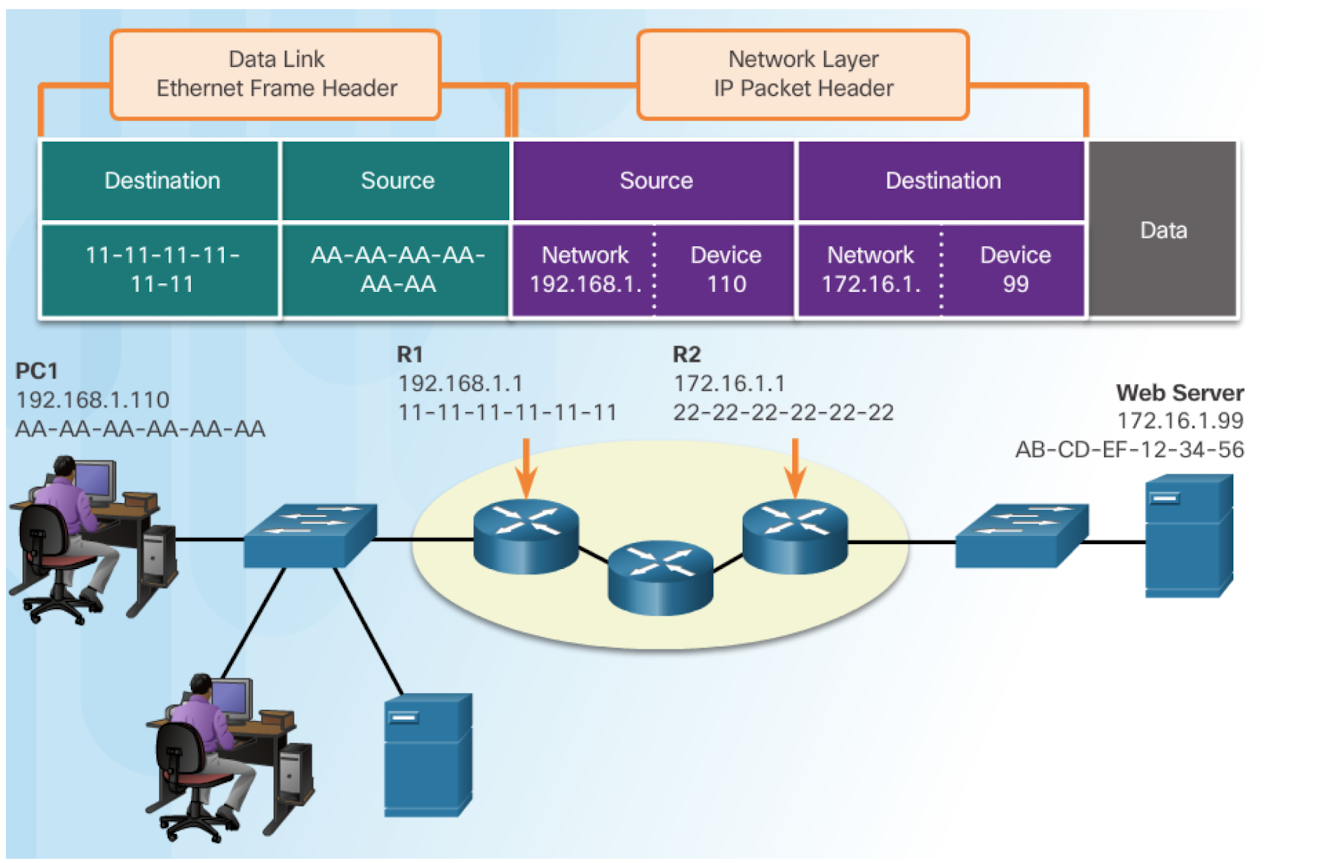
\includegraphics[width=12cm]{img/02_transport_data.png}
\end{center}

\newpage
\section{Schichten 1 und 2: Network Access}

\paragraph{Aufgaben Schicht 1}
Die physikalische Schicht (Layer 1) bietet der Sicherungsschicht (Layer 2) den Dienst an, Bits über einen Link zu übertragen. Ethernet umfasst Layer 1 und Layer 2.

\paragraph{Wichtigste Physikalische Schnittstellen an Netzelementen}

Folgende physikalische Komponenten werden standardisiert:
\begin{itemize}
\item Netzwerkanschlüsse (Network Interface Card -- NIC)
\item Übertragungsmedien (Leitungen)
\item Steckverbinder
\item Elektrische Signale
\item Kodierung
\end{itemize}


\paragraph{Drei wichtigste Übertragungsmethoden und deren Eigenschaften}

\begin{itemize}
\item \emph{Synchrone Übertragung} -- Das Taktsignal wird mit dem Datensignal mitübertragen
\item \emph{Asynchrone Übertragung} -- Nur das Datensignal wird übertragen. Der Empfänger benötigt eine \emph{Taktrückgewinnung}
\end{itemize}

Im Allgemeinen wird asynchron übertragen. Der Empfänger muss das Taktsignal aus dem Empfangssignal zurückgewinnen. Das Ziel ist es, \emph{1)} so viele Daten pro Zeiteinheit wie möglich und \emph{2)} so weit wie möglich zu übertragen. Die Dämpfung elektrischer Signale in einem Leiter nimmt i.A. mit der Frequenz zu.

Das Empfangssignal ist ein analoges Signal. Der Empfänger entscheidet um welches Symbol es sich handelt. Dabei können Fehler auftreten.

\paragraph{Wichtigste Kabel und wie sie eingesteckt werden}
\begin{itemize}
\item \emph{Unshielded Twisted-Pair Cable} -- Verschiedene Kabel mit verdrillten Kupferadern
\item \emph{Shielded Twisted-Pair Cable} -- Verschiedene Kabel mit verdrillten Kupferadern; abgeschirmt
\item \emph{Coaxial cable}
\end{itemize}



\begin{center}
\begin{tabular}{|m{1cm}| m{3cm} |m{2cm}|m{3cm}|} 
Medium& Eigenschaften & Vorteile & Nachteile\\ 
\hline
Kupfer & Twisted / Untwisted & Billiges Material & Dämpfung hoch bei hohen Frequenzen\\
Glas & Multimode (mehrere Pfade für das Licht), Singlemode (Pfad in eine Richtung) & Störungs-unabhängig, dämpfungs-arm & Teure Hardware\\
Luft & Signal wird auf Träger moduliert & Mobilität & Hohe Dämpfung bei hohen Frequenzen, alle können Signale empfangen und mithören, Interferenzen mit anderen Sendern, beschränkte Bandbreite wird geteilt\\
\end{tabular}
\end{center}


\paragraph{Leitungscode}

Der Sender wandelt das binäre Signal zuerst in einen dem Kanal angepassten Leitungscode um. Der Leitungscode legt fest, wie das Signal übertragen wird. Dabei ist es wichtig, das Signal dem Übertragungsmediom entsprechend anzupassen, um eine optimale Übertragung zu erreichen.

\paragraph{Aufgaben der Sicherungsschicht (data link layer)}

\begin{itemize}
\item Rahmenbildung um Pakete zu begrenzen
\item Regelung des Zugriffs auf den Übertragungskanal
\item Fehlererkennung
\item Optional (von Ethernet nicht unterstützt)
	\begin{itemize}
	\item Aufbau, Halten und Auflösen einer Verbindung
	\item Fehlerkorrektur durch Übertragungswiederholung
	\item Flusssteuerung
	\end{itemize}
\end{itemize}

Dafür werden Protokolle der Sicherungsschicht verwendet: \emph{LAN} -- Ethernet2, Ethernet IEE 802.3, TokenBus IEEE 802.4, Token Ring IEEE 802.5, WLAN IEEE 802.11; \emph{WAN} -- HDLC (High-Level Data Link Control), PPP, FrameRelay

\paragraph{Allgemeine Struktur eines Schicht-2-Rahmens}
Die Schicht 2 legt die Felder des Rahmens und die maximale Länge der Daten (Maximum Transmission Unit, MTU) in einem Rahmen fest.

\begin{center}
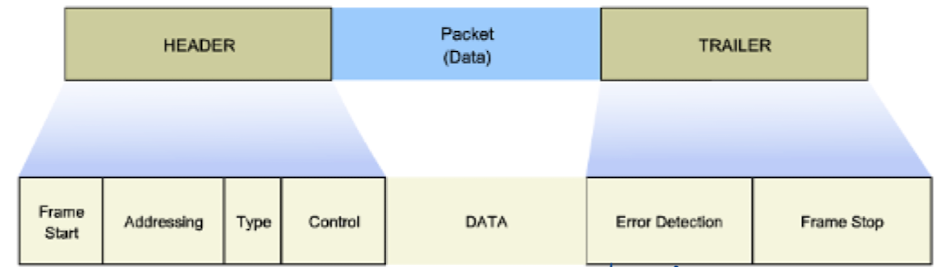
\includegraphics[width=12cm]{img/04_L2_frame.png}
\end{center}

\paragraph{Verschiedene logische Topologien in LAN}

\begin{itemize}
\item Stern
\item Erweiterte Stern
\item Bus
\item Ring
\end{itemize}

\begin{center}
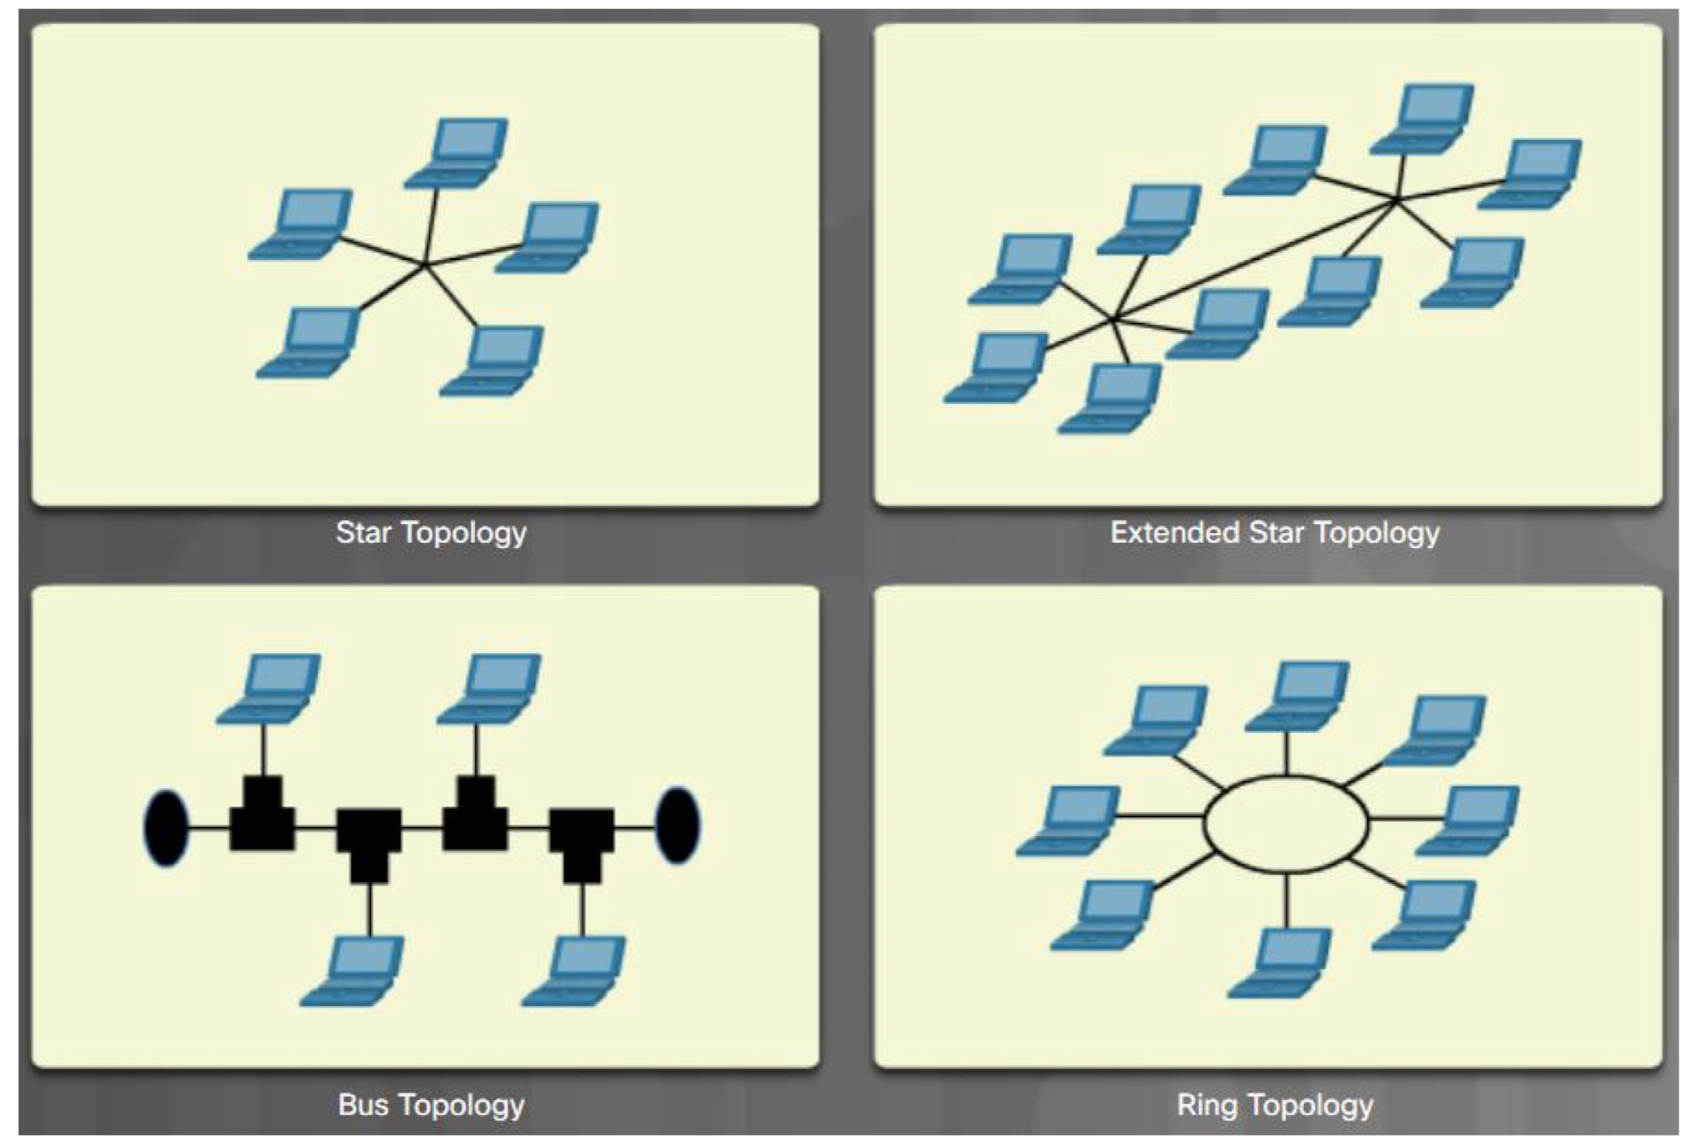
\includegraphics[width=12cm]{img/04_lan_topology.png}
\end{center}

\paragraph{LAN} Ursprünglich Shared Medium. Viele Stationen benützen denselben Kommunikationskanal. Weiterentwicklung: \emph{switched networks}

\emph{Half-Duplex} -- Ein Endgerät kann zu einem Zeitpunkt entweder senden oder empfangen (Ethernet mit einem Hub; Wireless Access Point)

\emph{Half-Duplex} -- Beide Enden können gleichzeitig senden und empfangen (Ethernet mit Switches).

\paragraph{Maximum Transmission Unit}
\begin{itemize}
\item Jedes L2-Protokolldefiniert eine MTU
\item Ein Rahmen darf nicht grösser sein als die MTU; ggf. muss das Schicht 3 Protokoll einen Rahmen fragmentieren, wenn er für einen Link zu gross ist
\item Typische MTU: 1500 Bytes
\item Grund: Ein Benutzer darf einen Kanal nicht zu lange belegen damit andere auch senden / empfangen können
\end{itemize}

\paragraph{Verschiedene logische Topologien in WAN}
\begin{itemize}
\item Punkt-zu-Punkt -- dedizierte Leitungen
\item Point-to-Multipoint -- Hub and Spoke, partial mesh; Hub Standort mit mehreren Standorten verbunden
\item Full Mesh -- Alle Geräte können miteinander kommunizieren
\item Ring -- Weniger anfällig auf Fehler wegen Verbindung im Kreis; kein single-point-of-failure
\item Stern -- nur zentraler Hub kann single-point-of-failure werden
\end{itemize}


\paragraph{Kategorien des Kanalzugriffsverfahren}
\emph{Controlled Access} -- Jede Station hat eine Zeit, die für sie zum Senden reserviert ist. In dieser Zeit darf nur sie senden (Token Ring, FDDI).

\emph{Contention-based Access} -- Als Wettbewerb: Der schnellere darf senden. Es ist ein Verfahren definiert, wie vorzugehen ist, wenn zwei Stationen gleichzeitig senden.

\newpage
\section{Ethernet}

\paragraph{OSI-Schichten von Ethernet abgedeckt} -- Ethernet deckt die Schichten 1 (Physikalisch) und 2 (Data Link, Sicherung) ab.

\paragraph{Aufgaben der MAC-Schicht}
\begin{itemize}
\item Kapselung der Daten
	\begin{itemize}
	\item Markierung des Beginns eines Rahmens
	\item Adressierung
	\item Fehler Detektion
	\end{itemize}
\item Kontrolle des Kanalzugangs
	\begin{itemize}
	\item Platzierung der Rahmen auf den Kanal
	\item Fehlerbehandlung bei Kollisionen
	\end{itemize}
\end{itemize}


\paragraph{Physikalische Unterlagen von Ethernet}
\begin{itemize}
\item Coax N-Style -- 500m
\item Coax BNC -- 185m
\item UTP RJ45 -- 100m
\item STP mini-DB-9 -- 25m
\item MM Fiber SC -- 220-550m
\item MM Fiber SC -- 550-5000m
\end{itemize}

\paragraph{Topologie vom ursprünglichen Ethernet}
\begin{itemize}
\item Offen
\item Einfachheit, einfacher Unterhalt, Zuverlässigkeit
\item Neue Technologien integrieren, ohne Alte ersetzen zu müssen.
\item Günstig in Installation und Aufrüstung
\end{itemize}

Mit Koaxkabel ("Bus") wurde das Ethernet ursprünglich entwickelt.

\paragraph{Kollisionsdomänen} -- Kollisionsdomänen werden unterteilt nach Geräten, die gleichzeitig senden / empfangen können. Wenn zwei Rechner in der gleichen Kollisionsdomäne sind, kann je nur einer der beiden gleichzeitig senden / empfangen.

Kollisionsdomänen können mit Hub erweitert (mehr Geräte einschliessen) und mit Switch oder Bridge in mehrere aufgetrennt werden.

\paragraph{Ethernet-Adressen} -- Allgemein werden entsprechend dem Adressaten drei Arten von Paketen unterschieden
\begin{itemize}
\item \emph{Unicast} -- Ziel ist ein Rechner
	\begin{itemize}
	\item Unicast-Adressen -- LSB des ersten Byte ist Null
	\end{itemize}
\item \emph{Multicast} -- Ziel ist eine Gruppe von Rechnern oder NIC
	\begin{itemize}
	\item Die IP-Adressen von 224.0.0.0 - 231.255.255.255 repräsentieren Multicast-Gruppen
	\item Wenn sich eine Anwendung an einer Multicast-Gruppe anmeldet, wird dem Rechner eine IP-Adresse vom Multicast-Bereich zugeordnet
	\item Zuordnung geschieht auf Schicht 3. Schicht 2 wird nachgezogen (Für IP-MC muss auch MAC-Adresse gebildet werden)
	\end{itemize}
\item \emph{Broadcast} -- Ziel sind alle NIC in einem Netz
	\begin{itemize}
	\item Ziel-Adresse lautet FF:FF:FF:FF:FF:FF
	\end{itemize}
\end{itemize}

\paragraph{Aufbau MAC-Adresse} -- MAC-Adressen bestehen aus zwei Teilen (je 3x 2 Oktet). Somit werden die ersten 6 Oktet der dem Hersteller (Organisationally Unique Identifier, OUI) vergeben. Der zweite Teil kann der Hersteller frei vergeben (Vendor Assigned; NIC, Interfaces)

Es gibt $2^{48}$ mögliche MAC-Adressen. Eine Organisation kann also $2^{24}$ verschiedene MAC-Adressen generieren.


\paragraph{Normen für Ethernet}
Als Standards werden hauptsächlich \emph{IEEE 802.3} und \emph{Ethernet2} verwendet.


\begin{center}
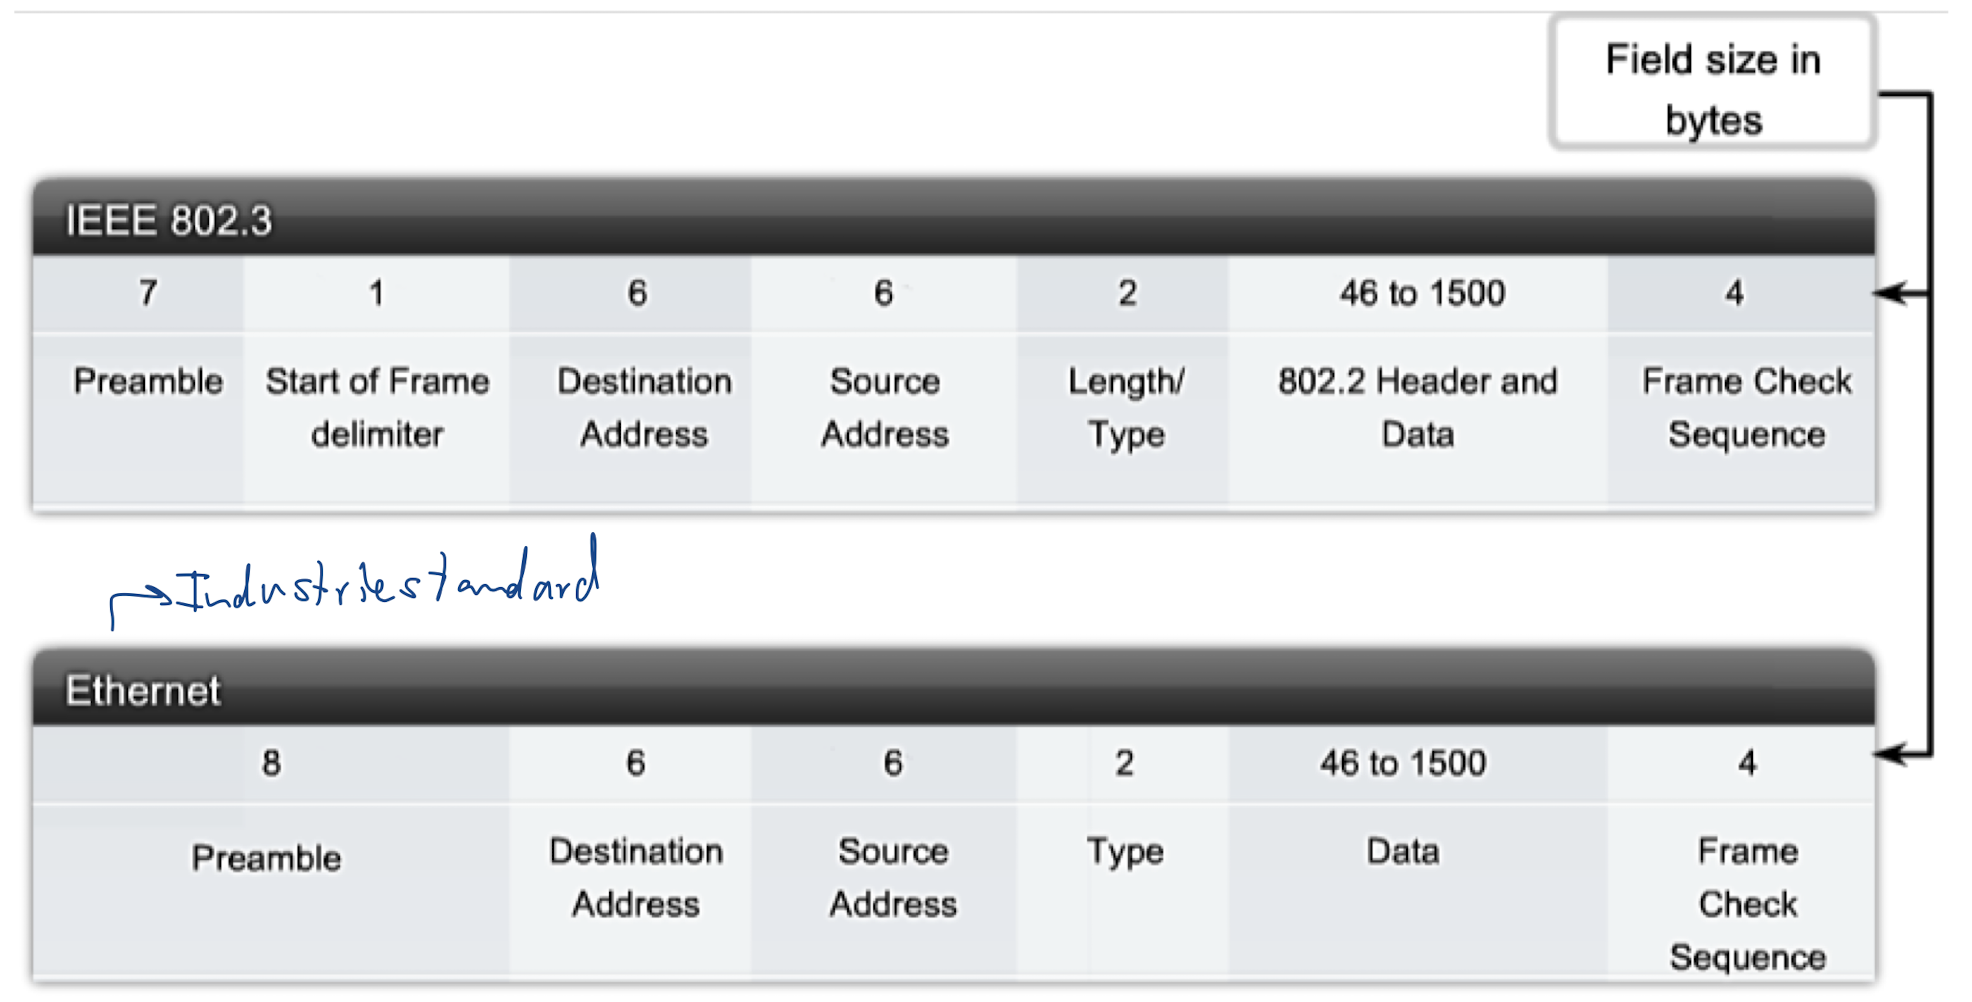
\includegraphics[width=12cm]{img/05_Ethernet_Rahmen.png}
\end{center}

Die Definition eines Ethernet-Rahmens impliziert, dass sie eine MTU (1500 Bytes) und eine Minimum Transmission-Unit (46 Bytes).

Anhand Byte 13 und 14 kann unterschieden werden nach welchem Standard, der Rahmen aufgebaut ist:
\begin{itemize}
\item Inhalt $>$ 0x0600: Ethernet2
\item Inhalt $<$ 0x0600: IEEE 802.3
\end{itemize}

Das Netzwerk-Interface prüft bei jedem Rahmen, wie er interpretiert werden muss. Bei IEEE-Rahmen folgt auf das Feld Length/Type das Feld LLC (3 Byte). LLC enthält den Protokollcode für das innere Protokoll der Payload. Alle IEEE 802.n-Normen haben das gleiche LLC-Feld.



\paragraph{Kanalzugriffsverfahren für Ethernet}
Carrier Sense Multiple Access / Collision Detection: Eine Station, die senden möchte, hört zuerst, ob der Kanal frei ist. Wenn Kanal frei ist, darf gesendet werden. Dabei kann es zur Kollision kommen.

Eine Kollision muss sicher von jeder Station detektiert werden. Bei einer Kollision: \emph{1)} Senden des Jam-Signals; \emph{2)} Rückzug vom Kanal; \emph{3)} Station generiert Zufällige $n$ und wartet $n*t_s$ wobei $t_s$ die Slotzeit ist.
Dafür muss jeder Ethernet-Rahmen eine minimale Länge haben.

\paragraph{Repeater und Bridge}
Ein \emph{Repeater} ist ein elektrischer Verstärker in einem "shared medium". Segment 1 und 2 bleiben Verbunden und bilden somit eine Kollisionsdomäne.

Eine \emph{Bridge} macht Zwischenspeicherung von Rahmen in Layer 2. Somit wird in zwei Kollisionsdomänen aufgetrennt.

\emph{Multiport Bridge} -- Switch: Auftrennung in verschiedene Kollisionsdomänen.


\begin{center}
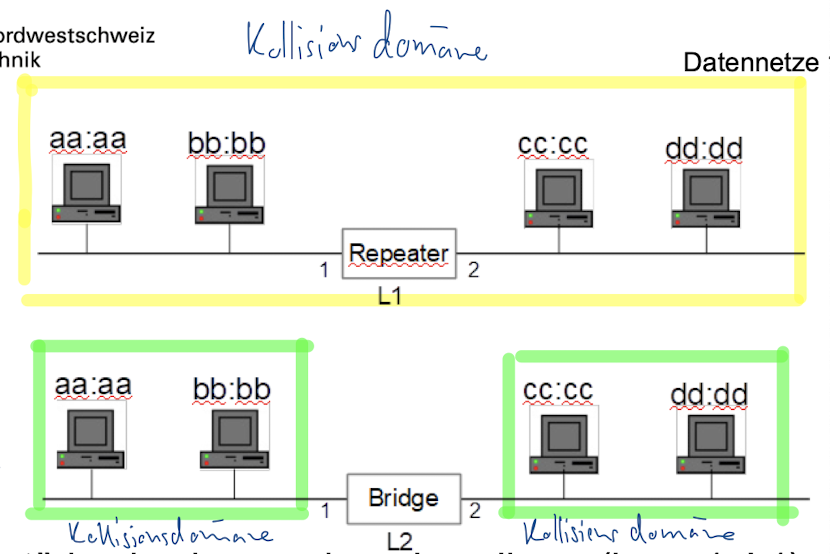
\includegraphics[width=12cm]{img/05_Bridge.png}
\end{center}


\paragraph{MAC-Tabelle} -- Lernen der MAC-Adressen: Switch merkt sich für jeden ankommenden Rahmen den \emph{Eingangsport} und die \emph{Absenderadresse}. Die Absenderadresse wird in die entsprechende Zeile eingefüllt.
Nicht mehr auftretende MAC-Adressen werden wieder gelöscht.

Anhand der Tabelle werden ankommende Rahmen weitergeleitet.

\paragraph{Hub und Switch} -- Weiterleitung von Ethernet-Rahmen

Auf Hub muss geprüft werden, ob Bus frei, dann kann gesendet werden. Wenn ein Switch verwendet wird, können alle senden und empfangen -- Switch handelt den Verkehr.

Ein Switch hat vier Operationen: \emph{1)} Learning (MAC-Tabelle), \emph{2)} Aging (nach ca. 2 Min ohne Auftreten wird ein Eintrag gelöscht), \emph{3)} Flooding, \emph{4)} Selective Forwarding \\

\emph{Flooding} -- Wenn Zieladresse von ankommendem Rahmen nicht in MAC-Tabelle: Rahmen wird an alle Ports (ausser Eingansport) weitergeleitet.

\emph{Selective Forwarding} -- Zieladresse ist in MAC-Tabelle: Rahmen wird nur an den entsprechenden Port weitergeleitet.

\newpage
\paragraph{Ablauf ARP}
Wenn der Quellrechner die Ziel-Adresse, aber nicht die Ziel-MAC-Adresse kenn wird die Zuordnung der MAC-Adresse zu einer IP-Adresse mittels \emph{Address Resolution Protocol} gemacht. Rechner und Router speichern die MAC-Adresse con Ziel-IP-Adressen lokal in der ARP Tabelle. Nach entsprechender Zeit werden die Einträge in der Tabelle entfernt (gealtert).

\emph{Probleme} -- Zu viel Broadcastverkehr; ARP-Spoofing (Attacker gibt sich als Default Gateway aus und kann so allen Verkehr mitlesen)


\newpage
\section{Netzwerkschicht} 
Von einem Netz ins andere und Protokolle IPv4, IPv6, AppleTalk, ICMP, OSPF und andere werden angewendet. Daten von Schicht 2 werden in Schicht 3 gekapselt.

\paragraph{Aufgaben Schicht 3}
\begin{itemize}
\item Adressierung
\item Kapselung in Senderichtung
\item Wegleitung -- Routing durch viele Netze
\item Entkapselung beim Empfang
\item Fehlerbehandlung
\end{itemize}

\paragraph{Eigenschaften IP}
Das Protokoll \emph{IP} ist:
\begin{itemize}
\item \emph{verbindungslos} -- Es werden IP-Pakete bei der Quelle los geschickt ohne, dass das Ziel davon weiss
\item \emph{best effort} -- Das Netz leitet soviele Pakete weiter, wie gerade möglich; Pakete werden weggeworfen bei Überlauf
\item \emph{Media independent} -- Läuft über allen möglichen Schicht 2 Protokollen (Ethernet, TokenRing, PPP, ATM) und Schicht 1 Medien
\end{itemize}



\paragraph{Header: IPv4} -- Der Header wird mit Zeilen à vier Byte dargestellt.

\begin{itemize}
\item \emph{Version} -- IP Version 4
\item \emph{IP Header Length} -- Header hat nicht immer Länge von 20 Bytes; wird in Anzahl Zeilen, $n*4$ Bytes angegeben
\item \emph{Differentiated Services} -- ursprünglich vorgesehen, Verkehr zu priorisieren -- wird nicht angewendet; kann in lokalen Services für QoS für e.g. Sprachanwendungen verwendet werden
\item \emph{Total Length} -- Länge des gesamten Paketes
\item \emph{Identification, Flag, Fragment Offset} -- werden (selten) verwendet, wenn Paket grösser als zulässige länge für Schicht 2 Protokoll (e.g. 1500 Bytes für Ethernet); Oft machen Implementationen der Transport Schicht (Layer 4) Segmente mit einer maximalen Länge von 1460 Bytes;
\item \emph{Time-to-live} -- Zahl dekrementiert bei jedem Hop; wenn TTL=0 wird das Paket verworfen und über ICMP Meldung an Absender; wird benötigt, damit Pakete nicht unendlich lange kreisen
\item \emph{Protocol} -- gibt an, welchem Protokoll ein angekommenes IP-Paket übergeben werden soll
\item \emph{Header Checksum} -- Paket wird verworfen, wenn Checksum nicht korrekt
\item \emph{Source IP Address} -- Adresslänge 4 Bytes
\item \emph{Destination IP Address} -- Adresslänge 4 Bytes
\item \emph{Options} -- wird oft nicht verwendet;
\item \emph{Padding} 
\end{itemize}

\paragraph{Header: IPv6}
\begin{itemize}
\item \emph{Version} -- Inhalt ist 6
\item \emph{Traffic Class (4 bit)} -- ursprünglich vorgesehen, Verkehr zu priorisieren -- wird nicht angewendet; kann in lokalen Services für QoS für e.g. Sprachanwendungen verwendet werden
\item \emph{Flow Label (20 bit)} -- Spezial-Dienst für Echtzeitanwendungen; Information an die Router, den selben Pfad für den Strom beizubehalten; Pakete müssen an Ziel nicht geordnet werden
\item \emph{Payload Length (16 bit)} -- Länge des ganzen IP-Paketes; exklusive Header und Extension Header
\item \emph{Next Header (8 bit)} -- Gibt das Protokoll an, das auf den IPv6-Header folgt
\item \emph{Hop Limit (8 bit)} -- Wird bei jedem Router dekrementiert. Erreicht es $0$ wird das Paket verworfen und es wird eine ICMPv6 Meldung an Quelle gesendet (Paket nicht an Ziel angekommen)
\item \emph{Source IP Address (128 bit)}
\item \emph{Destination IP Address (128 bit)}
\end{itemize}


\paragraph{Was macht ein Router mit einem eingehenden Paket?} -- Paket wird anhand der Routing-Tabelle weitergeleitet



\paragraph{Funktion von Default Gateway} -- Ein Default Gateway muss an jedem Rechner (der nach aussen kommunizieren soll), auf jedem Switch (der aus anderen Netzen angesprochen werden soll) und auf jedem Router konfiguriert werden.

Das Default Gateway wird beim Rechner entweder manuell oder per DHCP-Server definiert.\\Auf Switch: \verb+S1(config)#ip default-gateway 192.168.10.1+



\paragraph{Funktion von Routing-Tabelle} -- Es kann zwischen Routing-Tabelle auf Rechner und Router unterschieden werden. 

In der Routing-Tabelle auf dem Rechner wird das Loopback Interface (127.0.0.1), das lokale Netz und eine Default-Route eingetragen. Für die Default-Route muss das Default Gateway konfiguriert sein. Wird entweder durch DHCP Server oder manuell gesetzt.
 
In der Routing-Tabelle auf einem Router werden direkt angeschlossene Netze, entfernte Netze (statische Einträge; dynamische Routingprotokolle) und die Default Route eingetragen





\paragraph{Aufbau Router; Prozess während Aufstarten}
Ein Router hat:
\begin{itemize}
\item CPU -- Weiterleitung Pakete; rechnet Routing-Algorithmus
\item RAM -- IOS wird nach Aufstarten in RAM geladen; enthält running-config; enthält Routing-Tabelle; enthält ARP-cache
\item ROM -- Diagnostic Software für Tests bei Aufstarten (POST: Power On Self Test); Speichert bootstrap BefehleM
\item Flash -- Permanente Speicherung IOS
\item NVRAM -- nichtflüchtiger Speicher für startup-config
\item mindestens 2 Netzwerk-Interfaces -- Anschlüsse
\end{itemize}

Beim Aufstarten wird \emph{1)} POST durchgeführt, \emph{2)} die bootstrap Befehle geladen, \emph{3)} das IOS lokalisiert und geladen, \emph{4)} und das configuration file lokalisiert und geladen.

Die Konfiguration wird entweder aus dem NVRAM oder von einem TFTP-Server geladen.



\paragraph{Zustände bei Router abfragen}
\begin{lstlisting}
Router#show ip interface brief // IF Zustand
Router#show ip route // Routing-Tabelle
\end{lstlisting}


\newpage
\section{IP-Addressierung}

\paragraph{IPv4: Adresse und Subnetzmaske}

\begin{itemize}
\item \emph{Netzadresse} -- Hat lauter Nullen im Hostteil (erste Adresse des Netzes)
\item \emph{Broadcastadresse} -- Hat lauter Einsen im Hostteil (letzte Adresse)
\item \emph{Hostdressen} -- alles zwischen Netz- und Broadcastadressen
\end{itemize}

Rechner- und Router-IFs erhalten \emph{immer} eine Hostadresse.

 

\paragraph{IPv4: Unicast, Multicast und Broadcast} -- Es gibt drei verschiedene Arten von Ziel-Adressen:
\begin{itemize}
\item \emph{Unicast} -- Ein IP-Paket geht an genau ein IF. In einem /24-er Netz sind dies die Adressen 1 bis 254
	\begin{itemize}
	\item Werden auf Rechner entweder über DHCP-Server oder manuell eingerichtet
	\end{itemize}
\item \emph{Broadcast} -- Ein Rechner stellt eine Anfrage mit lauter Einsen im Hostteil (255)
\item \emph{Multicast} -- Pakete an eine Gruppe von Rechnern senden; 224.0.0.0 - 239.255.255.255; 224.0.0.0 - 224.0.0.255 nur link-lokal und werden nicht geroutet; 224.0.1.0 - 239.255.255.255 sind globale Multicast Adressen
	\begin{itemize}
	\item Hilft bei Verteilung eines Datenstroms; Sender sendet Pakete nur einmal und Switch/Router leiten Pakete an jeweilige Ports weiter
	\end{itemize}
\end{itemize}

\paragraph{Unterscheiden: Öffentliche und Private Adressen} -- Es sind drei Adressräume für private Verwendung vorgesehen: 10.0.0.0/8; 172.16.0.0/12; 192.168.0.0/16

Private Adressen werden im öffentlichen Internet nicht weitergeleitet.

\paragraph{Spezielle Adressen}
\begin{itemize}
\item 127.0.0.1 -- Loopback (127.0.0.1/8 ist reserviert)
\item 169.254.0.0/16 -- Link-lokale Adressen; können automatisch dem "Local Host" zugewiesen werden
\item 192.0.2.0/24 -- Unterricht und Dokumentation
\item 240.0.0.0/4 -- ist reserviert und darf nicht gebraucht werden
\end{itemize}
	
	
\paragraph{Klassenbezogene und Klassenlose Adressierung} -- Ursprünglich wurde der IPv4 Adressbereich in fünf Klassen unterteilt (A-E). Mit der Netzklasse wird nicht die tatsächliche Grösse eines Netzes angegeben, sondern wie viele Adressen es umfassen kann.
\begin{itemize}
\item A -- 0.0.0.0 - 127.255.255.255; 0 + 7 bit Netz, 24 bit Host;128 Netze; 16'777'214 Hosts pro Netz
\item B -- 128.0.0.0 - 191.255.255.255; 10 + 14 bit Netz, 16 bit Host; 16'384 Netze; 65'534 hosts
\item C -- 192.0.0.0 - 223.255.255.255; 110 + 21 bit Netz, 8 bit Host; 2'097'150 Netze; 254 Hosts pro Netz
\item D -- 224.0.0.0 - 239.255.255.255 (Multicast Gruppe); 1110 + 28 bit Multicast-Gruppen-ID
\item E -- 240.0.0.0 - 255.255.255.255 (reserviert; wird nicht genutzt); 1111 + 28 bit
\end{itemize}

Mittlerweile ist diese Technologie veraltet und es wird mit Subnetzmasken definiert, welchen Adressbereich ein Netz abdeckt. Dies nennt man klassenlos oder Classless Inter-Domain Routing (CIDR).

\paragraph{IPv6: Adressierung, Struktur mit Präfix. Subnet-ID und Interface-ID}
Mit der Einführung von IPv6 wird \emph{1)} ein grösserer Adressraum eingeführt  \emph{2)} hierarchische Vergabe der Adressen unterstützt \emph{3)} eine feste Headerlänge definiert  \emph{4)} das ICMP verbessert und  \emph{5)} Network Address Translation (NAT) abgeschafft.

IPv6-Adressen bestehen aus einem Prefix und einer Interface ID. Diese sind definiert durch "/n" nach der Adresse, wobei es n-bit des Prefixes definiert. 2001:0DB8:000A::/64 entspricht also 2001:0DB8:000A:0000 (prefix) :0000:0000:0000:0000 (Interface ID)

\paragraph{Übergang IPv4 zu IPv6} -- Mit tunneling von IPv6-Inseln über ein IPv4-Netz können IPv6-Netze miteinander sprechen.

\paragraph{Dual-Stack} ist, wenn IPv4 und IPv6 koexistieren. Dabei laufen beide Protokolle parallel. Wenn beide Enden IPv6 unterstützen, läuft Kommunikation über IPv6, ansonsten über IPv4.

\paragraph{IPv6 Adressen}
\begin{itemize}
\item \emph{Unicast} -- Ein Empfänger
	\begin{itemize}
	\item Global -- 2000::/3; weltweig eindeutig; Im Internet geroutet
	\item Link-Local -- weden nur lokal verwendet; FE80::/10
	\item Loopback -- Logisches IF zum eigenen IPv6 Stack; ::1/128
	\item Unspecified -- kann verwendet werden, wenn Quelle irrelevant ist
	\item Unique/Site Local -- Nicht verwenden für Kommunikation ins Internet; Für Kommunikation in Firmennetzen
	\item Embedded -- IPv4 kompatible Adressen für IPv4-IPv6 Translation
	\end{itemize}
\item \emph{Multicast} -- eine Gruppe von Empfängern
\item \emph{Anycast} -- Eine unicast Adresse, die Gruppen von Network IFs zugewiesen wird; Das Paket wird an das nächste IF weitergeleitet
\end{itemize}

\paragraph{IPv6 Unicast Adressen}
\begin{itemize}
\item \emph{Global Routing Prefix} -- Regional Internet Registry vergibt Adressen aus dem Adressraum 2000::/3; ISP erhält /32er-Adressbereiche; ISP geben Kunden /48er oder kleinere Netze;
\item \emph{Subnet ID} -- Adress-Teil vom 49. bis zum 64. bit
\item \emph{Interface ID} -- 64 letzte bit; entsprechen Host-Teil von IPv4; Rechner kann mehrere IPv6-Adressen auf einem physikalischen IF haben
\end{itemize}

Auf Cisco Router muss IPv6-Routing eingeschaltet werden:
\begin{lstlisting}
// IPv6 Routing einschalten
R1(config)#ipv6 unicast-routing 

// Interface fa0/0 mit IPv6 Adresse konfigurieren
R1(config)#interface fa0/0
R1(config-if)#ipv6 address 2001:db8:acad:1::1/64
R1(config-if)#no shutdown

// Kontrolle
R1#show ipv6 interface brief
R1#show ipv6 route // Routing Tabelle
    // Spezifische Adresse pingen (Verbindung testen)
R1#ping 2001:db8:acad:10::5
\end{lstlisting}

\paragraph{ICMPv4/v6} -- Mit dem Internet Control Message Protocol kann überprüft werden, ob in einem Netzwerk das Routing soweit stimmt, dass Rechner A den Rechner B in einem anderen Netz erreichen kann.

Die wichtigsten ICMP Meldungen sind:
\begin{itemize}
\item Host confirmation mit echo request und echo response -- feststellen ob ein Host erreichbar ist (ping, traceroute)
\item Destination or Service Unreachable -- Router sendet Nachricht an Absender, wenn er ein Paket nicht weiterleiten kann, weil er keinen passenden Eintrag in der Routingtabelle findet.
\item Time exceeded -- TTL auf null; Fehlermeldung zurück an Absender
\item Route redirection -- Router kann einem direkt angeschlossenen Rechner sagen, dass es einen schnelleren Weg gibt als über diesen Router
\end{itemize}

Protokoll-Stack von ICMPv4 ist [L2-Header $|$ IP $|$ ICMP] -- L2 Header ist meistens ein Ethernet Header; ICMP ist Schicht-3-Protokoll (benützt Dienste von Schicht 3 aber nicht höhere).

Bei ICMPv6 wird zudem \emph{1)} Router Solicitation Meldungen (RS),  \emph{2)} Router Advertisments (RA) \emph{3)} Neighbour Solicitation (NS) und \emph{4)} Neighbour Advertisment (NA) durchgeführt.
RS und RA werden für die Autokonfiguration bei IPv6 verwendet. NS und NA werden für Address resolution (IPv4 ARP) und Duplicate Address Detection verwendet.

\emph{Neighbour Solicitation für Adress Resolution} -- Station sendet eine ICMPv6 NS Meldung zu einer IPv6 Adresse, um zugehörige MAC-Adresse zu finden.

\newpage
\section{Unterteilen und Zusammenfassen von IP-Netzen}
Da der IPv4-Adressraum rasch knapp wurde, hat man begonnen Adressraum wo möglich zu sparen. Netze wurde nur so gross gemacht, wie nötig -- man hat begonnen IPv4-Netze zu unterteilen.

Zudem ist es sinnvoll, nicht zu grosse Netze zu haben. Jede Station verursacht Broadcast-Anfragen. Viele Hosts in einem Netz machen viel Broadcast-Verkehr.

Mit der Unterteilung von IPv4-Netzen kann dem entgegengewirkt werden.

\paragraph{IPv4-Netz in gleich grosse Subnetze unterteilen} -- Netze können halbiert werden, um in gleich grosse Subnetze unterteilen.
Beispiel: 192.68.1.0/24 in zwei Netze
\begin{itemize}
\item 192.68.1.0/25
\item 192.68.1.127/25
\end{itemize}
Somit wurde das ursprüngliche Netz in zwei gleich grosse Subnetze unterteilt. Anzahl Subnetze pro Netz ist jeweils eine 2er-Potenz.

Anzahl nutzbare Host-Adressen ist $2^{32-n} - 2$ -- also 2er-Potenz minus Netzadresse und Broadcast-Adresse

\paragraph{IPv4-Netz in verschieden grosse Subnetze unterteilen} -- Für WAN-Netze werden /30er Netze verwendet! Diese werden oft ans Ende des Adressraumes gesetzt.


\paragraph{Berechnungen mit Subnetzmasken variabler Länge}
Geeignete Subnetzmasken bei variabler Grösse:
\begin{itemize}
\item Bis 126 Hosts -- 255.255.255.128
\item Bis 62 Hosts -- 255.255.255.192
\item Bis 30 Hosts -- 255.255.255.224
\item Bis 14 Hosts -- 255.255.255.240
\item Bis 6 Hosts -- 255.255.255.248
\item Bis 2 Hosts -- 255.255.255.252 (kann für WAN verwendet werden)
\end{itemize}

\setlength{\tabcolsep}{10pt}
\renewcommand{\arraystretch}{1.2}


Beispiel:
\begin{center}
\begin{tabular}{|m{2cm}| m{0.5cm} |m{2.8cm}|m{2cm}|m{2cm}|} 
Netzname & \#  & Subnetzmaske & Netzadresse & Broadcast-Adresse\\
\hline
Sales Office & 40 & 255.255.255.192 & 172.16.0.0 & 172.16.0.63\\
Technical Support & 35 & 255.255.255.192 & 172.16.0.64 & 172.16.0.127\\
Engineering & 30 & 255.255.255.192 & 172.16.0.128 & 172.16.0.191\\
HR & 23 & 255.255.255.224 & 172.16.0.192 & 172.16.0.223\\
Executive Mgmt & 10 & 255.255.255.240 & 172.16.0.224 & 172.16.0.239\\
WAN1 & - & 255.255.255.252 & 172.16.0.240 & 172.16.0.243\\
WAN2 & - & 255.255.255.252 & 172.16.0.244 & 172.16.0.247\\
WAN3 & - & 255.255.255.252 & 172.16.0.248 & 172.16.0.251\\
WAN4 & - & 255.255.255.252 & 172.16.0.252 & 172.16.0.255\\
\end{tabular}
\end{center}

\setlength{\tabcolsep}{18pt}
\renewcommand{\arraystretch}{1.2}

Daraus resultieren die Netze:
\begin{itemize}
\item 172.16.0.0/26
\item 172.16.0.64/26
\item 172.16.0.128/26
\item 172.16.0.192/27
\item 172.16.0.224/28
\item 172.16.0.240/30
\item 172.16.0.244/30
\item 172.16.0.248/30
\item 172.16.0.252/30
\end{itemize}


\paragraph{Netze in IP-Adressräumen zusammenfassen}
Die Zusammenfassung muss den gleichen Adressraum bedecken, wie die einzelnen Netze.


\paragraph{Adressraum sinnvoll einteilen und planen}

Zudem wird empfohlen bei der Belegung eines Adressraumes nach einem ähnlichen Muster zu folgen. Beispiel:
\begin{center}
\begin{tabular}{|m{4cm}| m{1cm} |m{1cm}|} 
Engerät & Von & Bis\\
\hline
Router / Switch & .1 & .15\\
Andere Netzwerkgeräte & 16 & .23\\
Server & .24 & .31\\
Clients & .32 & .240\\
Reserve & .241 & .255\\
\end{tabular}
\end{center}

\paragraph{Entwurfsleitlinien für IPv6} -- IPv6-Netze immer gleich gross wählen: /64

\newpage
\section{Transportschicht}

\paragraph{Aufgaben der Transportschicht (Schicht 4)} 
\begin{itemize}
\item Multiplexierung
\item Falls grosse Datenblöcke erwartet werden:
    \begin{itemize}
    \item Segmentierung und Wiederzusammensetzen von grossen Datenblöcken
    \item Sicherung der Übertragung (fehlerfreie Übertragung)
    \item Flusssteuerung
    \end{itemize}
\end{itemize}

\emph{Multiplexierung} -- Die Datenströme werden beim Empfänger entsprechend der Anwendung zugeordnet. Gewisse Anwendungen (e.g. für Filetransfer) senden / empfangen grosse Datenblöcke.

\emph{Segmentierung} -- Wenn ein Datenblock grösser als die MSS (Maximum Segment Size) ist, segmentiert das Transport-Protokoll die Daten und verpackt jedes Segment einzeln in ein IP-Paket. Segmente werden beim Zielrechner wieder zusammengesetzt.

\paragraph{Anforderungen von Anwendungen an die Kommunikation} Es gibt Anwendungen, welche grosse und andere die kleine Datenblöcke senden. Dafür werden zwei Protokolle unterschieden:

\emph{TCP} -- Verbindungsorientierte, fehlerfreie Übertragung; viel Overhead -- kann also langsam werden; Anwendungen benötigen einen zuverlässigen Dienst

\emph{UDP} -- Anwendungen mit Nachrichten kürzer als die MSS; verbindungslos -- schnell; Jedes Datagramm wird am Ziel einzeln und sofort der Anwendung abgeliefert;

\paragraph{Protokolle in Schicht 4}


\subsection{TCP}

\paragraph{TCP (Header und Bedeutung der Felder)}


\paragraph{Verbindungsaufbau TCP}

\paragraph{Schwachstellen TCP}


\subsection{UDP}
macht keine Flusskontrolle
\paragraph{UDP (Header und Bedeutung der Felder)}

\paragraph{Fehlerkorrektur}

\paragraph{Flusssteuerung}

\paragraph{Vorteile und Gefahren UDP}











\section{}


\end{document}












